\tableofcontents
\newpage
\section{Einführung}
Der Mensch unterliegt genauso den natürlichen Gesetzen wie alle anderen Lebewesen auf unserer Erde. Somit ist es logisch, dass auch der Mensch dem Drang der Fortpflanzung unterliegt, um das Bestehen der Art der Menschen auch in der Zukunft zu gewährleisten. Dieser Effekt lässt sich am besten mit dem immerwährenden Anstieg der Anzahl der auf der Erde lebenden Menschen betrachten. Schon seit tausenden von Jahren ist der Trend ganz klar ausschließlich positiv, und es gab nur wenige Ausnahmen davon, die allerdings im Wesentlichen immer auf Ereignisse heruntergebrochen werden können, die keinen Ursprung in der Natur haben. Dazu zählen Kriege, andere zwischenmenschliche Auseinandersetzungen, Krankheiten und Naturkatastrophen. Biologisch ist die Fortpflanzung einer Art maßgeblich durch die Ressourcen oder eben deren Abwesenheit beschränkt. Mit der Entwicklung des modernen Menschen hat sich eben dies dahingehend verändert, dass der Mensch nicht mit der natürlichen Ressourcenregulation unterliegt. Jedenfalls betrifft es den Menschen auf einer anderen Abstraktionsebene. Somit ist der Mensch in der Lage, wenn er denn genug von Nahrungsmitteln hat, sich im Prinzip unendlich weiter fortzupflanzen. Dies bringt nun allerdings eine Reihe von Problemen mit sich. In dieser Arbeit wird die Möglichkeit beleuchtet, das Problem eines eventuellen Nahrungsmangels in der Zukunft zu bekämpfen, indem ein moderner Ansatz der Nahrungsmittelproduktion erschaffen wird. Dazu werden hierbei insbesondere sogenannte Vertical Farms betrachtet. Die moderne Marktwirtschaft zeigt einen Trend auf, der sich in die Richtung solcher Farmen bewegt. Der Grund dafür mag vielfältiger Natur sein, lässt sich allerdings durch die Standortunabhängigkeit und Kosteneffizienz wohl am besten zusammenfassen. Diese Arbeit versucht nun, eine Metrik zu etablieren, die nicht nur beschreibt, inwiefern sich Vertical Farms in einer Skalierung verhalten, sondern gibt auch noch ein Beispiel dazu, wie komplex etwaige Systeme sind und wie viele einzelne Komponenten von Interesse sind. Dazu wurde im Laufe dieses Projekts ein neuronales Netz implementiert, welches das Alter von Setzlingen und Jungpflanzen anhand von Bildern prognostizieren kann.
\begin{figure}
    \centering
    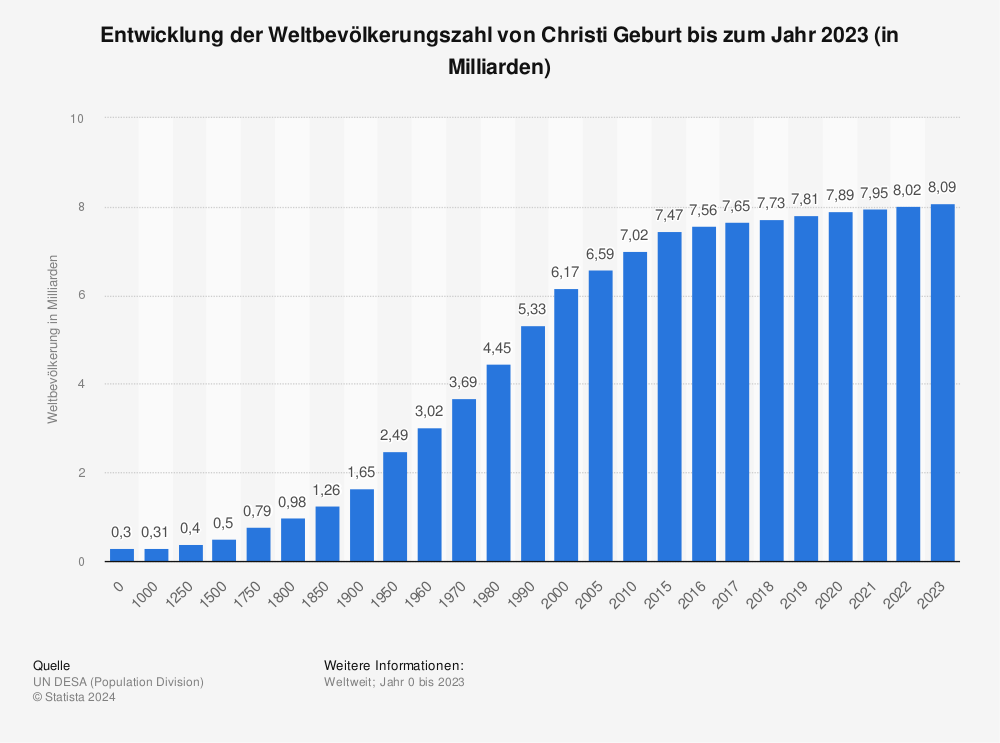
\includegraphics[width=1\linewidth]{1694.png}
    \caption{Entwicklung der Weltbevölkerung}
    \label{fig:enter-label}
\end{figure}
\subsection{Nahrungsmittel und Ressourcen}
Der Mensch nutzt seit Anbeginn seiner allgemeinen Intelligenz die Ressourcen der Erde, um seine Lebensgrundlage zu gewährleisten. Hauptsächlich hat er dafür Pflanzen angebaut, da die Fauna zwar auch eine Nahrungsmittelquelle darstellt, aber auf die benötigte Masse berechnet, nur einen kleinen effizienten Teil ausmachen kann. Daher hat der Mensch sich früh darauf konzentriert, Pflanzen derart anzubauen, um möglichst viel Gewinn für sich erschaffen zu können. Dazu musste er eine Reihe von Techniken entwickeln, um den Maßstab des Anbaus vergrößern zu können. 
\subsection{Steinzeit und früher Mensch}
Zunächst fing er damit an, Pflanzenteile nicht direkt von dem jeweiligen Wirt zu essen, sondern sammelte größere Mengen einer Pflanze, um sie dann entweder einzulagern oder auch Pflanzen, die eher feingranular dargereicht werden, verzehren zu können. Dazu zählen zum Beispiel auch Beeren, welche nur relativ wenig an einem Strauch vorhanden sind, aber beim Sammeln durchaus eine sättigende Menge bereitstellen können. \cite{early}
\subsection{Beginne der Landwirtschaft}
Als mit dem Einzug von weiterer Intelligenz der Mensch erkannte, wie der Prozess des Samenursprungs in der Botanik funktioniert, fing er an, Pflanzen an gezielten von ihm auserwählten Standorten anzubauen und so die Wege, die er davor auf sich nehmen musste, einzusparen. Zunächst war das Wissen der einflussreichen Faktoren, die das Pflanzenwachstum beschränken und steuern, sicherlich gering, weswegen zur damaligen Zeit noch nicht besonders große Erträge zu rechnen waren. Als der Mensch dann aber durch den fortschreitenden iterativen Lernprozess den Prozess des Anbaus immer weiter optimierte, kamen immer mehr Faktoren dazu, die beachtet wurden und so die Produktivität erhöhen konnten. Beispielsweise sind die Beachtung von Sonnenstand und Grundwasser extrem signifikant für das Wachstum einer Pflanze. So ist aus frühen archäologischen Funden klar geworden, dass der Mensch alsbald erkannte, dass Pflanzen in Tälern wesentlich besser wachsen als auf Hügeln und steinigem Boden. Bald darauf entwickelten sich erste rudimentäre Äcker, auf denen gezielt eine Monokultur von Pflanzen angelegt wurde. Diese wurden dann nachweislich auch mit Werkzeugen, die speziell für den Ackerbau erfunden und entdeckt wurden, bewirtschaftet. Somit muss also klar gewesen sein, dass nicht nur natürliche Gegebenheiten, sondern auch das direkte Einwirken und Verfahren des Anbaus hochgradig relevant sind für den Erfolg. Mit der Erfindung weiterer Maschinen wurde immer mehr die körperliche Arbeitslast des Menschen minimiert, ohne einen direkt negativen Einfluss auf die Produktivität der landwirtschaftlichen Mission zu haben. Spätestens dann, mit der Erfindung der Dampfmaschine sowie des allgemeinen Motors, war es nun nicht mehr notwendig, Felder händisch zu bestellen, sondern einzelne Personen konnten mit einem Mal Flächen verarbeiten, für die es vormals dutzende, teils hundert Arbeitskräfte benötigte. \cite{inproceedings}
\subsection{Industrialisierung}
Der wohl größte Umbruch für die Produktivität des Menschen war der Beginn des Zeitalters der Industrialisierung. Diese Zeit war gekennzeichnet von der extrem schnellen Entwicklung von Gerätschaften, Prozessen und Verfahren, die dazu führten, dass eine gigantische Lawine von Modernisierungsprozessen in Gang gebracht wurde, sodass es den Umfang des heutigen Verständnisses wahrscheinlich sprengen würde. Davon war natürlich auch die Landwirtschaft betroffen und die Anzahl an Menschen explodierte. Überall schossen Fabriken aus dem Boden, die die Nahrungsmittel verarbeiteten. Auch die Anzahl der monokulturellen Landwirtschaft stieg rasant an. Schnell wurde aber auch ein weiteres Problem offensichtlich, welches bis dahin kaum wahrgenommen wurde, beziehungsweise nicht in dem Maße beachtet wurde. Der Platz wurde knapp. Dieses Problem setzte sich bis in unsere heutige moderne Fort. Es bedarf heute mehr denn je einer Lösung, der Weltbevölkerung eine Möglichkeit der Ernährung zu bieten. \cite{Grünewald+2019+147+153} Mit der aktuellen Urbanisierung wird es außerdem immer schwerer, Fachkräfte zu etablieren, die sich dem Problem der Agrarwirtschaft widmen. Daher entwickelte sich zu Beginn der Jahrtausendwende ein Konzept. Das Konzept der Vertical Farm.

\section{Vertical Farming}
Vertical Farming beschreibt ein völlig neues Metakonzept, welches aktuell noch in den frühen Phasen der Entwicklung steht. Kernidee ist das fundamentale Konzept der Landwirtschaft, auf abstrahierten 2-dimensionalen Flächen die 3-Dimensionalität zu bringen. Dabei werden eine Vielzahl von Ansätzen verfolgt. Außerdem haben sich unter dem Oberbegriff "Vertical-Farming" nicht nur generelle Konzepte für angesprochene Semantik gesammelt, sondern auch eine Menge allgemeiner Modernisierungsansätze für intelligente Agrarwirtschaft entwickelt. So sind Dinge wie Smart-Farms und moderne Agrarwissenschaft stark in die Thematik verwoben. 
\begin{figure}
    \centering
    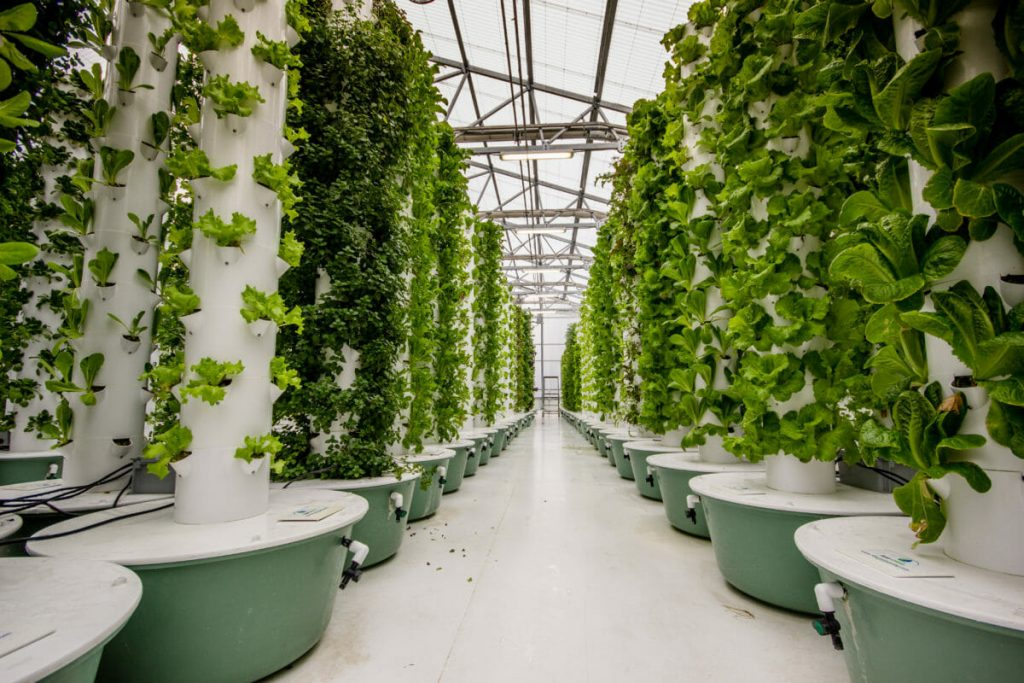
\includegraphics[width=0.9\linewidth]{aeroponics-1200x800-1-1024x683.jpeg}
    \caption{Hydroponische Vertical-Farm}
    \label{fig:enter-label}
\end{figure}
\subsection{Vertical-Farm Typen}
Das abstrakte Konzept von dreidimensionalem Farming hat unterschiedliche Auswüchse und Umsetzungen hervorgebracht. Im Rahmen dieser Arbeit wurde sich auf eine Anzahl von 5 Konzepten konzentriert, wobei erwähnt sei, dass es sich hierbei nur um einen kleinen Bruchteil der bereits in der Entwicklung befindlichen Ansätze handelt. Grundsätzlich unterscheiden sich die Konzepte vor allem auf der Ebene der konkreten Umsetzung, womit oftmals andere Faktoren wie zum Beispiel der Standort und der Energieverbrauch stark beeinflusst werden. \cite{agronomy12010002}
\subsubsection{Hydroponische Vertical-Farms}
Bei hydroponischen Vertical-Farms ist die grundsätzliche Idee, einen großen Verlustfaktor der Natur auszuschalten. Dazu wird in besagter Anbauform gänzlich auf die klassische Erde verzichtet. Stattdessen werden Pflanzen in einer Nährlösung subduziert, bei der die genaue Zusammensetzung bestimmt, gemessen und kontrolliert wird. Wie in Abbildung 2 zu erkennen ist, handelt es sich dabei um Polymerkonstrukte, die einer hochspezialisierten Bauweise unterliegen, um Sensorik und andere Optimierungen ermöglichen zu können. Dazu eignen sich fast alle Pflanzen, die einem schnellen Wachstum unterliegen. Allerdings können gewisse Arten auch Schäden davontragen, da beispielsweise die Pflanze nicht selbst ihre Wasseraufnahme reguliert, sondern vielmehr von externen Prozessen wie Regenfall gesteuert wird. Solche Pflanzen würden sich dementsprechend einer zu großen Menge Wasser bedienen, die so nicht von ihr verarbeitet werden kann. Allerdings kann somit auch auf feingranularster Ebene der Wasser- und Nährstoffhaushalt kontrolliert werden. So kann gerade in skalierbaren Anbau- und Systembedingungen eine signifikante Einsparung von Wasser erzielt werden. Eine Unterart der hydroponischen Systeme sind die aeroponischen Systeme, bei denen eben kein Wassersubstrat mehr zur Anwendung kommt, sondern vielmehr die Pflanze im Freien hängt und die Nährstoffe durch ein Aufsprühen mit einer entsprechenden Vorrichtung vorgenommen werden und somit ein sehr kontrollierbarer Düngevorgang vorgenommen werden kann. \cite{KANNAN20222163}
\subsubsection{Aquaponische Vertical-Farms}
\begin{figure}
    \centering
    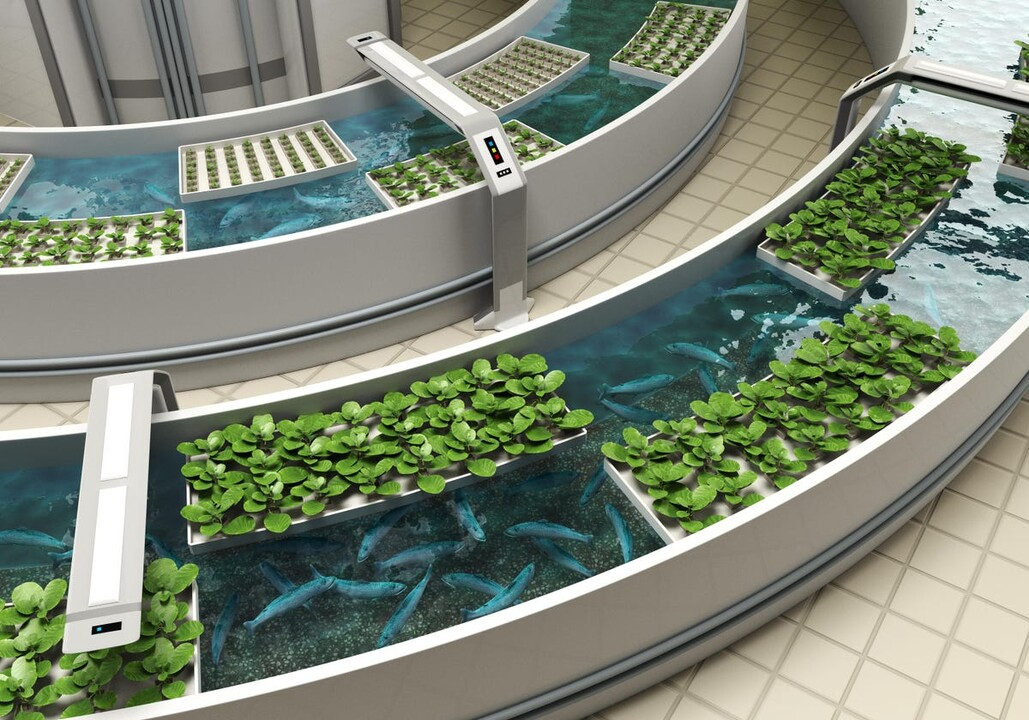
\includegraphics[width=0.9\linewidth]{1682655900899.jpg}
    \caption{Aquaponisches System (Modell)}
    \label{fig:enter-label}
\end{figure}
Aquaponische Systeme sind von besonderem Interesse in der modernen Agrarwirtschaft, da sie eine Vielzahl von Problemen adressieren, die sich in der Moderne gesammelt haben. Dazu zählt unter anderem die Tatsache, dass gewisse Lebensmittel nur noch schwerlich aus der Gesellschaft wegzudenken, geschweige denn zu entfernen sind. Genau genommen nehmen die aquaponischen Systeme einen wichtigen Stellenwert ein. Sie verbinden die Problematik der Fischzucht und die der komplexen Agrarwirtschaft, indem sie die beiden Systeme vereinen, um eine "Pseudosymbiose" zu schaffen. Wie in Abbildung 3 zu erkennen ist, befinden sich bei den meisten Systemen die Pflanzcontainer über einem Fischzuchttank, wodurch auch die Wege zwischen den beiden Komponenten möglichst klein gehalten werden sollen. Die grundlegende Idee ist, zwischen dem Fauna- und Florateil ein sich ergänzendes System zu schaffen. Dies kann natürlich in unterschiedlichster Art und Weise geschehen. Frühe Modellversuche dazu verwenden allerdings die Annahme, dass die Pflanzen Nährstoffe bereitstellen, von denen gewisse Fischarten profitieren können. Die Fische wiederum übernehmen die Funktion der Aufbereitung des Nährwassers für die Pflanzen und sorgen somit auch auf lange Sicht für eine kontinuierlich bessere Wasserqualität. Dabei entstehen somit auch zwei Ressourcen, die genutzt werden können. Einerseits der Fisch, der meist essbar ist, oder andere Ressourcen wie beispielsweise Fischöl erzeugt und eben auch die Pflanzen, die mit dem Wasser aus den Faunatanks bewässert werden. Zusammenfassend lässt sich hierbei vor allem erkennen, dass der Fokus auf der Ersparnis der Energie zur Aufbereitung des Nutzwassers liegt. Aber auch andere Faktoren lassen sich so deutlich besser kontrollieren, um eine Einsparung zu realisieren. Derartige Systeme befinden sich von allen in dieser Arbeit behandelten Systemen noch in der frühesten Entwicklungsphase. Grund dafür ist die wesentlich höhere Komplexität, die mit etwaigen Systemen einhergehen muss. Denn es wird nicht nur nach einer grundsätzlichen Möglichkeit gesucht, sondern auch nach einer Art und Weise, die nach erfolgreicher Entwicklung auf einen Umfang skaliert werden kann, der klassische Anbaumethoden ablösen könnte. \cite{OpportunitiesandChallengestoSustainabilityinAquaponicSystems}
\subsubsection{Container-Farming}
Im Vergleich zum aquaponischen Farming, welches wie bereits erwähnt einer Vielzahl von Faktoren und Problemen unterliegt, muss es auch Lösungen geben, die einfach umzusetzen sind. Dies ist vor allem dadurch zu begründen, dass solche Systeme weltweit zum Einsatz kommen sollen und somit an eine große Menge von Umgebungsbedingungen angepasst werden müssen. Dazu hat sich ein Ansatz entwickelt, bei dem vor allem der Fokus auf Skalierbarkeit gelegt werden soll. Dieser Ansatz wird im Allgemeinen als Container-Farming bezeichnet und beschreibt die Idee, kleine individuelle Einheiten zu schaffen, die sowohl einzeln als auch in einer großen Anzahl verwendet werden können, ohne große technische und standortbezogene Gegebenheiten verwenden zu müssen. Dabei werden alle notwendigen Systeme in dem Container verpackt und müssen autark funktionieren können. Dazu zählen Systeme wie Bewässerung, Stromversorgung für die Lampen, Sensortechnik und Rechner, die die Datenauswertung und Anpassungen vornehmen. Somit muss allerdings nicht nur eine Infrastruktur geschaffen werden, die die Funktionsfähigkeit des Containers innen erlaubt, sondern es muss eben auch ein System geben, welches eine hochskalierbare parallele Nutzung von etwaigen Containern erlaubt. Dazu muss beispielsweise ein Wasserleitungssystem gewährleistet sein, da es sich hierbei um eine Ressource handelt, die gezwungenermaßen von außerhalb des Containers kommen muss. \cite{SONG2023138353}
\begin{figure}
    \centering
    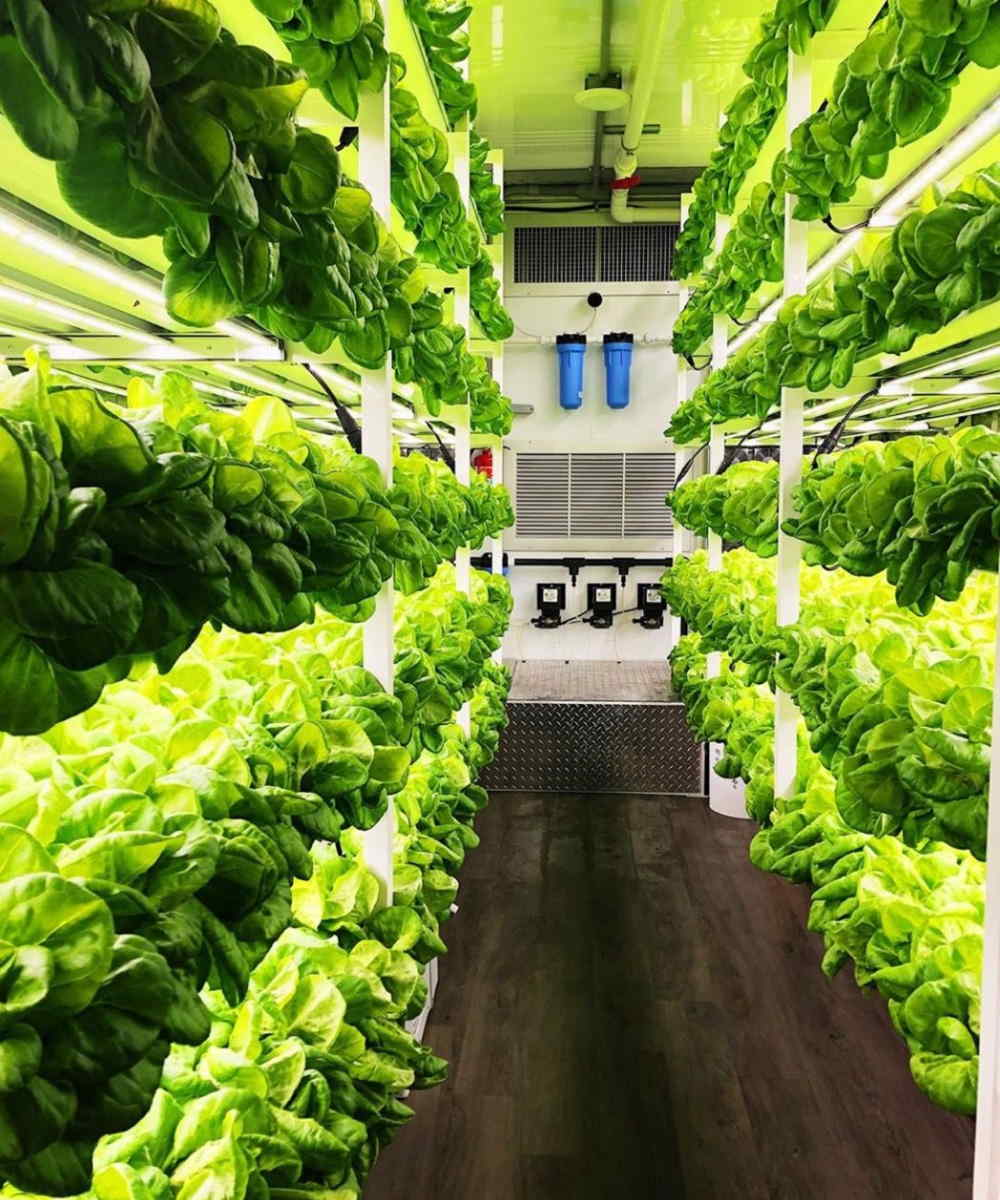
\includegraphics[width=0.7\linewidth]{thrive-container-farm-interior.jpg}
    \caption{Container-Farm mit Infrastrukturelementen}
    \label{fig:enter-label}
\end{figure}
\section{Biologische Grundlagen zum Projektteil}
\textit{Der folgende Teil der Arbeit wurde in Zusammenarbeit mit \textbf{Lina Jähnig} vom \textbf{Institut für Biochemie und Biologie} an der Universität Potsdam verfasst um eine biologisch fundierte Grundlage zu schaffen.}
\subsection{Wassertransport in der Pflanze}
Die Wasseraufnahme der Pflanze findet im Allgemeinen an der Wurzel bzw. der Wurzelspitze statt. Der Grund dafür ist, dass das Wasser an den Zellen der Wurzel ungehindert diffundieren kann. Das Wasser fließt daraufhin weiter in den Zentralzylinder im Wurzelschaft. Dort befinden sich die Gefäßelemente des Xylems. Das Xylem wiederum transportiert das Wasser von der Wurzel in die Blätter. Dies geschieht mit der sogenannten Massenströmung. Haupttreiber des Wasserflusses ist das Druckgefälle zwischen Blatt und Wurzel. Dabei besteht im Blatt ein Unterdruck im Verhältnis zum unteren Teil der Pflanze. Einerseits besteht der sogenannte Wurzeldruck, welcher das Wasser nach oben drückt, und andererseits ziehen die Blätter mittels des sogenannten Transpirationssogs das Wasser in die oberen Teile der Pflanze. Außerdem entsteht durch Osmose ein Konzentrationsausgleich von in dem Wasser gelösten Molekülen, die an den Blättern durch die Verdunstung von dem tragenden Wasser entstehen.\cite{urry2019}
\begin{figure}
    \centering
    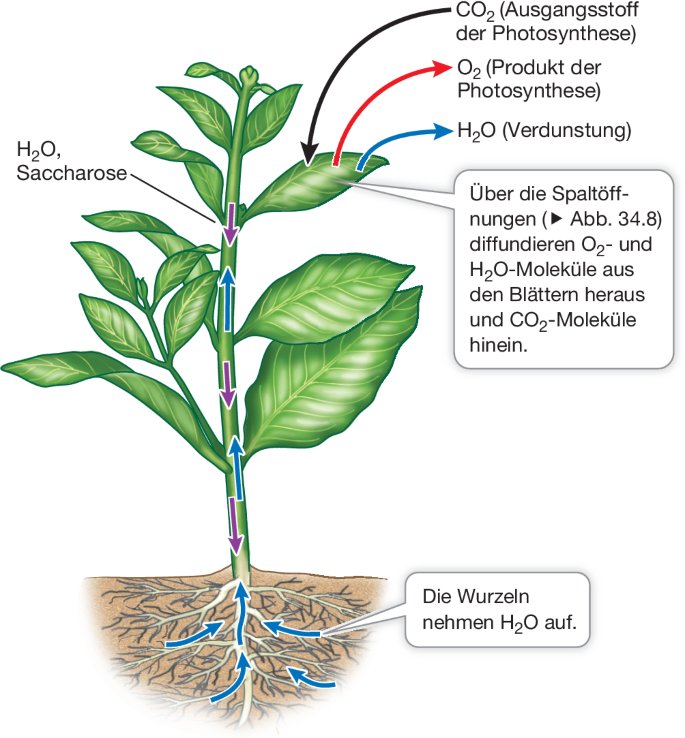
\includegraphics[width=0.5\linewidth]{154381_10_De_34_Fig1_HTML.png}
    \caption{Beispielhafter Wassertransport}
    \label{fig:enter-label}
\end{figure}
\subsection{Blattaufbau}
Die im Rahmen dieses Projekts behandelte Pflanze ist ein sogenannter Kormophyt. Dies sind alle höheren Pflanzen mit den folgenden 3 Grundorganen. Der \textbf{Wurzel}, der \textbf{Sproßachse} und das hier relevante seitliche Anhangsorgan, den \textbf{Blättern}. Die Blätter sind der zentrale Ort der Photosynthese und der Transpiration. Sie treten in vielen verschiedenen Formen und Varianten auf. Am häufigsten findet man das sogenannte bifaciale, dorsiventrale Laubblatt. Das bedeutet, die Ober- und Unterseite des Blattes sind morphologisch verschieden. Es existieren viele Sonderformen und Anpassungen an Umweltfaktoren.
\begin{figure}
    \centering
    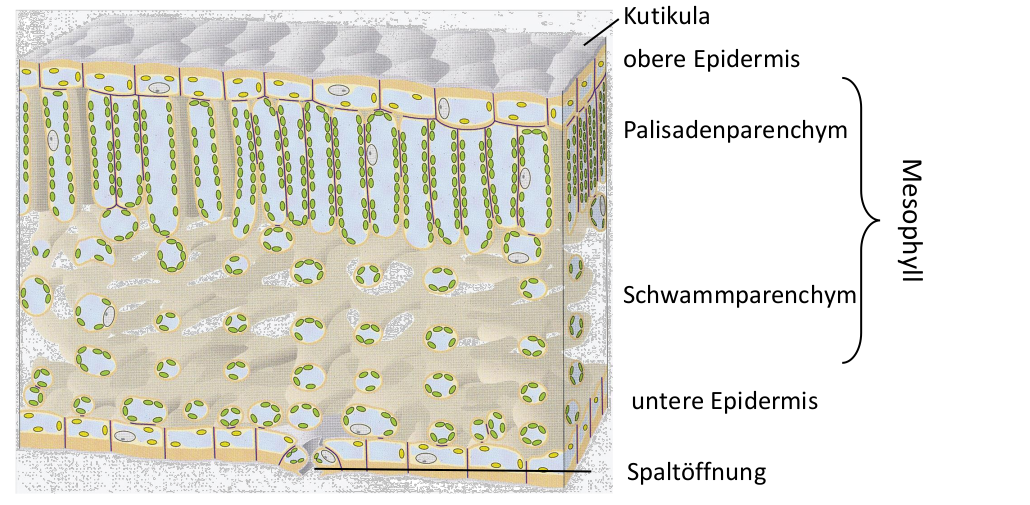
\includegraphics[width=0.7\linewidth]{Bildschirmfoto vom 2025-03-30 19-59-09.png}
    \caption{Querschnitt eines Laubblattes}
    \label{fig:enter-label}
\end{figure}
\subsubsection{Evolutionärer Hintergrund}
Das Blatt stellt einen evolutionären Vorteil gegenüber anderen photosynthese betreibenden Organismen dar. Landpflanzen vergrößerten ihre Blätter im Wettbewerb um Ressourcen, denn der Vorteil größerer und breiterer Blattflächen liegt in erhöhter Energieaufnahme über die Lichtabsorption. Der Nachteil jedoch ist ein erhöhtes Aufkommen von Evaporation.
\subsection{Wasser als grundlegende Ressource}
Ohne Wasser ist es Pflanzen im Allgemeinen nicht möglich, Fotosynthese zu betreiben, da ohne diese keine Reduktion des Kohlenstoffs stattfinden kann. Insbesondere bei Pflanzen ohne sekundäres Dickenwachstum, wie der hier relevanten Zuckerrübe, erhält der Wasserdruck in den Zellen die Ausformung der Pflanzenstruktur aufrecht. \cite{oeko}
\subsection{Wasserabgabe}
Pflanzen geben über alle Oberflächen Wasserdampf ab. Am meisten über die Spaltöffnungen der fotosynthetischen Organe. Landpflanzen unterliegen einer besonders starken Transpirationsbeanspruchung, weshalb die entsprechende Wasserzufuhr von außen gewährleistet sein muss. Die Wasserabgabe wird reguliert, indem die Schließzellen der Spaltöffnungen sensibel auf Wasserverlust reagieren. Junge Blätter transpirieren im Allgemeinen mehr Wasser als alte Blätter, da ihr wachsartiger Verdunstungsschutz, die Kutikula, weniger stark ausgebildet ist. Zudem wird die Transpiration durch äußere Faktoren begünstigt, wie beispielsweise die Luftfeuchtigkeit und Temperatur. Die Transpirationsrate kann außerdem auch über die Fläche des Blattes approximiert werden. Dazu wurden bisher aufwendige Versuche durchgeführt, in denen mittels chemisch-physikalischer Untersuchungen die Transpiration gemessen wurde. Derartige Systeme haben allerdings den Nachteil, dass nur ein relativ kleiner Bereich in die Messung einfließen kann. Diese Arbeit stellt also einen alternativen Ansatz vor, um die Anwendung besagter Datensammlungen zu verbessern bzw. deren Gültigkeitsbereich zu verallgemeinern.
\subsection{Zusammenfassung}
Zusammenfassend lässt sich also feststellen, dass die Pflanze auf Wasser angewiesen ist, da die oben beschriebenen Prozesse von einer möglichen Wasserzufuhr ausgehen. Die Hauptproblematik liegt nach dem aktuellen Stand darin, dass es keine direkt quantitative Analysemöglichkeit gibt, um die Wasseraufnahme zu bestimmen. \cite{exp} Die Blattfläche korreliert mit dem Wasserbedarf der Pflanze. Genau diesen Ansatz machen wir uns im Folgenden dieser Arbeit zunutze und verwenden die unten genannten Algorithmen, um die Brücke zwischen Messwert und Interpretation zu schließen.
\newpage

\section{Projektteil - ML-basierte Transpirationsflächen-Bestimmung}
Wie im vorherigen Kapitel erwähnt, ist die tatsächliche Transpirationsfläche der wohl stärkste Einfluss nehmende Faktor, wenn es um die Berechnung der theoretischen Wasseraufnahme geht. Die Wasseraufnahme ist für Vertical Farms von besonderer Relevanz. Wasser ist die Ressource, die nicht nur einer intensiven Aufbereitung bedarf, sondern sie ist auch meist mit größeren Kreislaufsystemen gekoppelt, die in sich auch wieder ressourcenaufwendig sind, viel Energie kosten und meist einer intensiven Wartung bedürfen. Daher ist es von besonderem Interesse, so wenig wie möglich an Wasser aufzuwenden, ohne große Einbußen am Ertrag der Nutzpflanze hinnehmen zu müssen. In Bezug auf Kapitel 2.1 ist die genauere Wasserkontrolle beispielsweise für die containerbasierten Vertical Farms von großem Nutzen. Wie bereits erwähnt, sind es eben diese Systeme, die zwar gut und vor allem sinnvoll skalierbar sind, aber eben einer gewissen Infrastruktur bedürfen, um ausreichend Wasser zur Verfügung zu stellen. \newline \par
Um nun genauer bestimmen zu können, wie viel Wasser einer Pflanze zur Verfügung gestellt werden muss, beschäftigt sich dieses Projekt damit, Bilderkennung zu verwenden, um die Transpirationsfläche der Pflanze zu bestimmen, womit wiederum die genaue Wassermenge, die der Pflanze im Rahmen der Bewässerung zugeführt wird, genau abgestimmt werden kann. Ein Großteil der, wie im Kapitel 1 beschriebenen, landwirtschaftlichen Anbaumethoden bewässert unabhängig vom Wachstumsstadium die Pflanzen meist mit der gleichen Wassermenge. Ein Großteil dieses Wassers kommt somit allerdings nicht mit der Pflanze in Kontakt, beziehungsweise wird von dieser verwendet, sondern versickert meist viel eher im Boden und geht wieder ins Grundwasser ein. Somit ist die Energie, die zum Abpumpen und Gießen verwendet wurde, im Prinzip verschwendet gewesen. Dieses Problem möchten wir, wie im Folgenden beschrieben wird, umgehen, indem wir die zugeführte Wassermenge der Pflanze abhängig von der genauen Blattfläche machen.
\subsection{Datensatz und Modellpflanze}
Damit eine sinnvolle Implementierung eines Neuronalen Netzwerks erfolgen konnte, war die erste wichtige Aufgabenstellung gewesen, einen geeigneten Datensatz zu finden, der wie im Folgenden zum Trainieren und Validieren des Modells verwendet werden kann. Dazu fiel die Wahl auf den \textbf{V2 Plant Seedlings} Datensatz, der im Jahre 2019 von der \textbf{University of Pretoria} in Südafrika erstellt wurde. Der Datensatz umfasst vor allem Nutzpflanzen und beinhaltet eine Reihe von Bildern der jeweiligen Pflanzen in unterschiedlichen Entwicklungsstadien und vor allem Altern. Im Verlaufe des Projekts fiel darin die Wahl auf den Datensatz der Zuckerrübe. \newline \par
Die Zuckerrübe ist seit langer Zeit hochgradig relevant als Nutzpflanze für die Menschheit, da sie von Natur aus einen sehr hohen Gehalt an verschiedenen Zuckern hat. Unter diesen Zuckern befindet sich auch die Saccharose, welche besonders interessant ist für den Menschen, da es sich dabei um eine Mischform der klassischen Zuckersorten Glukose und Fruktose handelt. Es bedarf nur weniger Arbeitsschritte, um aus der Zuckerrübe nutzbaren klassischen Haushaltszucker herzustellen. Wie in Abbildung 7 gut zu erkennen ist, bilden Zuckerrüben eine typische Blattform. Ansonsten handelt es sich bei der Zuckerrübe um eine Rübenart, was bedeutet, dass sich nach einem bestimmten Entwicklungsstadium eine dicke wurzelartige Form bildet.
\begin{figure}
    \centering
    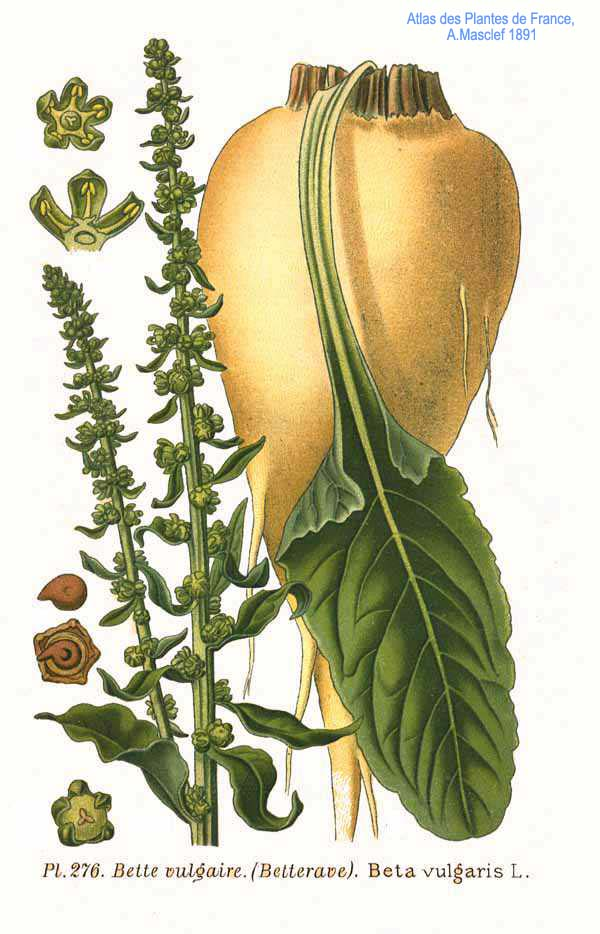
\includegraphics[width=0.4\linewidth]{276_Beta_vulgaris_L.jpg}
    \caption{Zuckerrübe der Gattung Beta vulgaris}
    \label{fig:enter-label}
\end{figure} 
\newline \par
Der Datensatz beinhaltet Bilder der immer gleichen Größe und vor allem wurde darauf geachtet, das Bild auf einen gleichen Seitenabstand zwischen Blattrand und Bildrand zu schneiden. Dies bietet eine umso bessere Grundlage, um den Datensatz zum Trainieren eines neuronalen Netzes zu verwenden. Außerdem wurden die Bilder fast vollständig mit dem gleichen Hintergrund aufgenommen, was abermals eine Konsistenz schafft, die es dem Modell leichter macht, tatsächliche Features zu erkennen. Insgesamt umfasst der Datensatz 463 Bilder von unterschiedlichen Zuckerrüben-Setzlingen, womit ein ausreichend großer Datensatz für eine primitive regressive Bildanalyse vorliegt. In den Abbildungen 8, 9 und 10 sind drei Beispielbilder aus dem Trainingsdatensatz gezeigt, die die Setzlinge in den drei grob relevantesten Phasen zeigen. Vorerst wird der Setzling aus dem Samenkorn nur sehr wenig Transpiration betreiben, da ein Großteil der Energie noch aus dem Samenkorn stammt. Mit der weiteren Entwicklung jedoch steigt die Photosynthese massiv an und die Transpirationsfläche wächst nach dem Modell einer gedeckelten Exponentialfunktion an. Die Transpirationsfläche wurde von zwei Personen anhand der Bilder schätzungsweise gebildet und entsprechend als Datenpunkt für das spätere Training vermerkt.
\begin{figure}
    \centering
    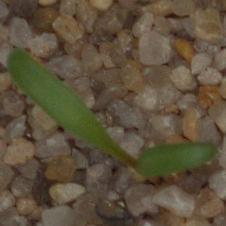
\includegraphics[width=0.6\linewidth]{4.png}
    \caption{Frühe Pflanze (Alter 1-4 Tage)}
    \label{fig:enter-label}
\end{figure}
\begin{figure}
    \centering
    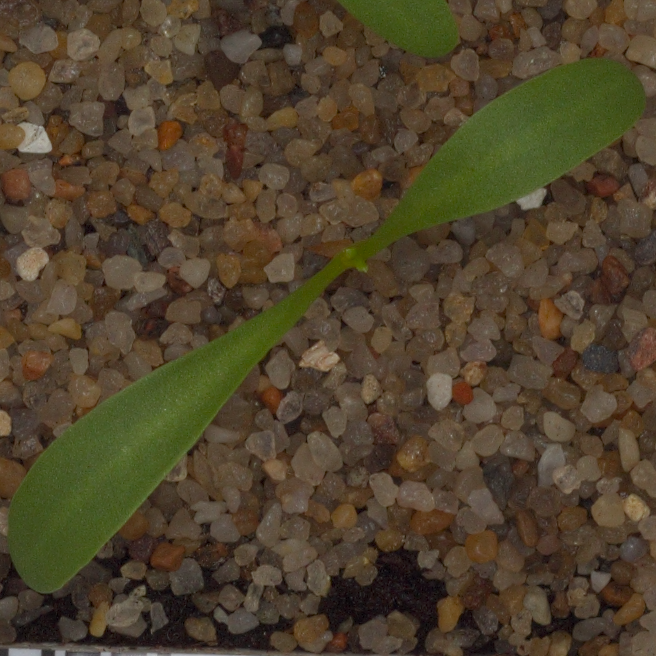
\includegraphics[width=0.6\linewidth]{60.png}
    \caption{Pflanze kurz vor weiterem Blattwachstum (Alter 14-28 Tage)}
    \label{fig:enter-label}
\end{figure}
\begin{figure}
    \centering
    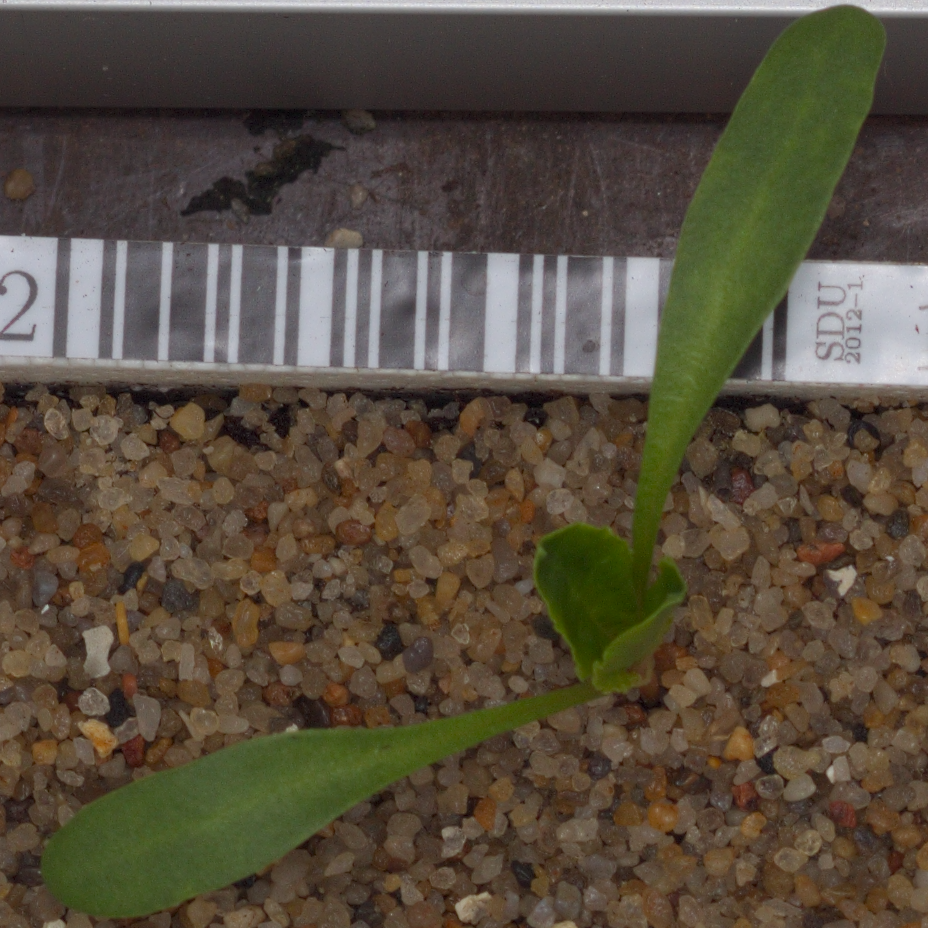
\includegraphics[width=0.6\linewidth]{444.png}
    \caption{Weitere Blätter entstanden (Alter 30 Tage+)}
    \label{fig:enter-label}
\end{figure}
\subsection{Theoretische Grundlage}
Um eine Regressionsanalyse, also eine Zahl als Ausgabe des Neuronalen Netzwerks zu erhalten, muss vorerst geklärt werden, ob sich ein derartiges Problem überhaupt eignet, um mit einem Neuronalen Netzwerk gelöst zu werden. Dies wird aber relativ schnell klar ab dem Zeitpunkt, wenn man mit Bildern als Eingabedaten arbeitet. Der Grund dafür ist, dass Bilder einen sehr großen Eingabevektor bilden, da sie sowohl x- und y-Koordinaten als auch RGB-Werte in Form von Ganzzahlen zwischen 0 und 255 besitzen. 
\[r, g, b \in \mathbb{N}\] für \[0 \leq r, g, b \leq 255\]
So würde sich ein Eingabevektor der Größe
\[G = S_x * S_y * r * g * b\] bilden, der aufgrund seiner extremen Größe kaum für klassische deterministische Algorithmen geeignet ist. 
Dabei sind:
\begin{itemize}
    \item $S_x$ die Größe des Bildes an der x-Achse,
    \item $S_y$ die Größe des Bildes an der y-Achse,
    \item $r$ Grundfarbwert für Rot,
    \item $g$ Grundfarbwert für Grün,
    \item $b$ Grundfarbwert für Blau
\end{itemize}
\subsubsection{Neuronale Netze}

Neuronale Netze sind ein Modell des maschinellen Lernens, das von der Struktur und Funktionsweise biologischer Nervensysteme inspiriert ist. Sie bestehen aus künstlichen Neuronen, die in Schichten organisiert sind: einer Eingabeschicht, einer oder mehreren versteckten Schichten und einer Ausgabeschicht. Jedes Neuron verarbeitet Eingaben, gewichtet sie und gibt ein Signal weiter, das durch eine Aktivierungsfunktion transformiert wird. \cite{Jansson1991}
Ein Neuron in einem künstlichen neuronalen Netzwerk wird durch eine gewichtete Summe seiner Eingaben aktiviert, gefolgt von einer Aktivierungsfunktion:

\begin{equation}
    z = \sum_{i=1}^{n} w_i x_i + b
\end{equation}

Dabei sind:
\begin{itemize}
    \item $x_i$ die Eingaben des Neurons,
    \item $w_i$ die entsprechenden Gewichte,
    \item $b$ der Bias-Wert,
    \item $n$ die Anzahl der Eingaben.
\end{itemize}

Die Aktivierung erfolgt dann durch eine nichtlineare Aktivierungsfunktion $\sigma(z)$, zum Beispiel die Sigmoid-Funktion:

\begin{equation}
    a = \sigma(z) = \frac{1}{1 + e^{-z}}
\end{equation}

Andere gängige Aktivierungsfunktionen sind die ReLU-Funktion:

\begin{equation}
    a = \max(0, z)
\end{equation}
und der hyperbolische Tangens:

\begin{equation}
    a = \tanh(z) = \frac{e^z - e^{-z}}{e^z + e^{-z}}
\end{equation}
\subsection{Neuronale Modellkomposition}
\begin{figure}
    \centering
    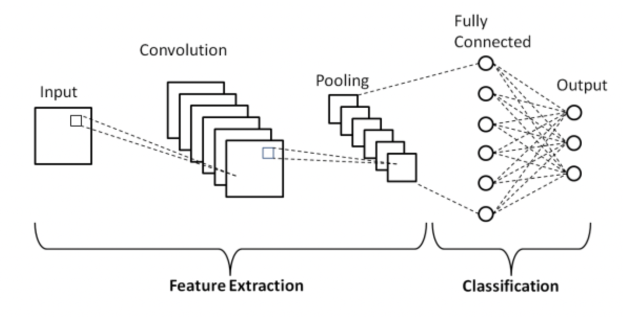
\includegraphics[width=1\linewidth]{1_-FR6rFrKXktjxwDTlGofPQ.png}
    \caption{Aufteilung des Neuronalen Netzes in Feature Extraction und Classification}
    \label{fig:enter-label}
\end{figure}
\begin{figure}
    \centering
    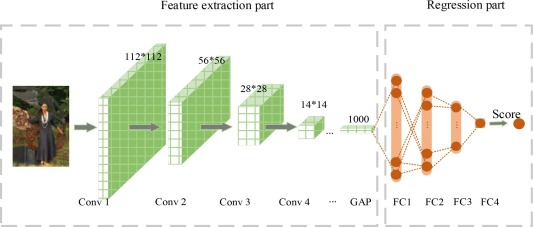
\includegraphics[width=1\linewidth]{1-s2.0-S1047320322002280-gr2.jpg}
    \caption{Faltungsfilterung zur Regressionsanalyse}
    \label{fig:enter-label}
\end{figure}
Über die letzten Jahre haben sich durch den massiven Aufschwung des Forschungsinteresses eine Vielzahl von neuronalen Netzarchitekturen gebildet, die sich meistens für bestimmte Zwecke besonders gut eignen. Bei der Bildanalyse hat sich aus der Vergangenheit gezeigt, dass es sehr sinnvoll ist, das Analysemodell in zwei grundlegende Teile zu unterscheiden. So wird das Modell in einen Teil für die Merkmalserkennung und einen Teil für die tatsächliche Gewichtung der Merkmale hin zu einer Regressionsanalyse strukturiert. Eine Faltung lässt sich im Prinzip sehr gut erklären, wenn man sich der Parallele zur tatsächlichen Pixeleinheit bewusst wird. Bei einer Faltung wird nun nicht einfach der Pixelwert in die nächste Instanz übertragen, sondern es wird viel eher der Kontext, also der Wert der umliegenden Pixel mit in die Auswertung einbezogen. Dadurch entsteht eine Kontextualität, welche dazu führt, dass bestimmte Features anders erscheinen, als sie es im ursprünglichen Bild getan hätten. Schemenhaft ist das Ganze in Abbildung 11 zu erkennen. Wichtig ist hierbei zu erwähnen, dass Features nicht nur auf einer Ebene direkt erkannt werden, sondern vielmehr ein Zusammenwirken von mehreren Faltungslayern ist. \cite{ZOU2024107839} Dabei kann man sich die Analogie vorstellen, dass auf frühen Layern erst einmal nur abstrakte Features erkannt werden. Beispielsweise bei einer theoretischen Erkennung von einem Menschen werden zunächst alle Gliedmaßen beurteilt, ohne jedoch einen korrekten Zusammenhang eines Körpers feststellen zu können. Erst auf späteren Faltungslayern wird dann sichergestellt, ob sich die jeweiligen Gliedmaßen auch an der richtigen Stelle befinden. Ähnliches ist auch für den untersuchten Datensatz von Relevanz. Dabei kann durch die Faltung ein Blatt identifiziert werden. Somit kann schon leicht quantifiziert werden, wie viele Blätter die Pflanze hat, was wiederum offensichtlich mit der Transpirationsoberfläche der Pflanze korreliert. Zusätzlich korreliert natürlich auch die Transpirationsfläche mit dem Alter der Pflanze. Dies wird im späteren Kapitel dieser Arbeit behandelt. \newline \par
Abbildung 12 zeigt eine sehr typische Bildanalyse, welche allerdings sehr gut in das Bild dieser Arbeit passt, da im Gegensatz zu Abbildung 11 hier keine Klassifikation verwendet wird, sondern vielmehr eine Regression. Modellhaft ist es genau diese Architektur, die auch bei diesem Projekt verwendet wurde. Auch der Übergang zwischen Faltungsanteil und voll verbundenen Layern ist sehr ähnlich gestaltet. Dabei wird im Prinzip ein flacher Feature-Vektor übergeben, welcher dann vom linearen Teil "interpretiert" wird. \cite{Lai_2019}
\newline \par
Das Modell, welches für dieses Projekt verwendet wurde, besteht aus insgesamt 7 Layern. Drei der Layer befinden sich im Teil der faltungsbasierten Filterung. Die restlichen 4 Layer der linearen vollverbundenen neuronalen Netzlayer befinden sich im Regressionsteil, in dem bei einem 1024-elementigen Eingabevektor in das erste Layer eingegeben wird. Das nächste Layer besitzt allerdings nur noch 64 Neuronen, das darauf folgende 32 Neuronen und das vorletzte nur noch 16 Neuronen. Schließlich befindet sich im letzten Layer des Modells nur noch ein Neuron, welches unsere Regressionsausgabe bildet. Die realwertige Ausgabezahl entspricht somit der Schätzung für die abgebildete Transpirationsfläche.
\subsection{Implementierung}
Für die Implementierung des Neuronalen Netzes wurde im Rahmen dieser Arbeit das Framework PyTorch ausgewählt. PyTorch zeichnet sich vor allem durch seine Performance und extrem gute Bedienbarkeit aus. Außerdem ist es mittlerweile sehr weit verbreitet und wird von vielen der aktuellen Forschungsprojekte wie zum Beispiel den Sprachmodellen von DeepSeek R1 verwendet. Zudem ist die Community um das Open Source Projekt sehr aktiv und bildet eine große fortschrittliche Gemeinschaft.
\subsubsection{Modellquellcode}
\begin{figure}
    \centering
    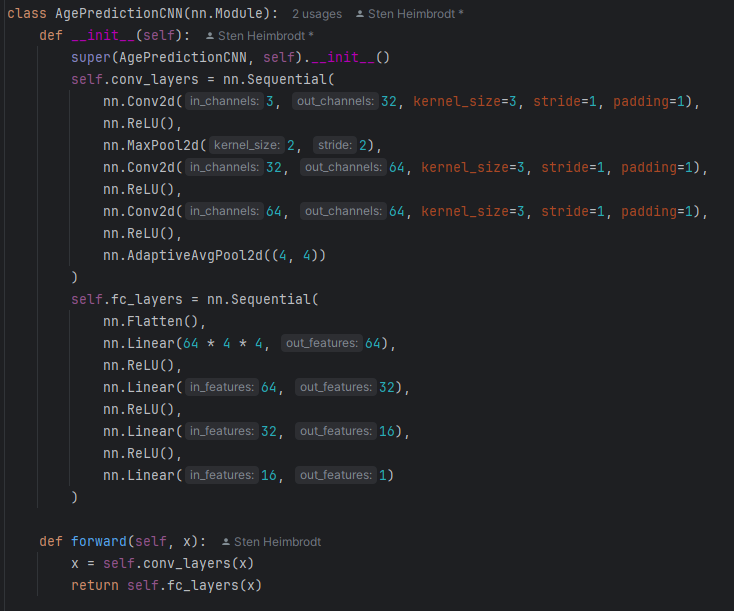
\includegraphics[width=0.9\linewidth]{Screenshot 2025-03-30 164658.png}
    \caption{Modellquellcode für die Regressionsanalyse}
    \label{fig:enter-label}
\end{figure}
In Abbildung 13 ist der vollständige Quellcode für das verwendete Modell zu sehen. Dazu sei kurz erwähnt, dass ich PyTorch die entsprechende Syntax zum Anlegen von Netzwerk-Layern extrem einfach finde. Letztendlich werden in Klassenkomponenten Listen angelegt, in denen eine Reihe aus intrinsischen Objekten liegen, in denen wiederum die einzelnen Layer definiert werden. Schlussendlich muss nur eine \textbf{forward} Funktion definiert werden. Mit dieser findet somit die letztliche Inferenz statt. Dabei ist bemerkenswert, wie einfach die Syntax gehalten werden kann, obgleich die Expressivität davon unberührt bleibt. So ist es den Entwicklern auch ein leichtes, an den Modellparametern zu variieren, ohne große syntaktische Hürden bewältigen zu müssen. Insgesamt kann so auch die Entwicklungsgeschwindigkeit von Machine Learning Modellen gesteigert werden.

\subsubsection{Trainingsimplementierung und Trainingserfolg}
\begin{figure}
    \centering
    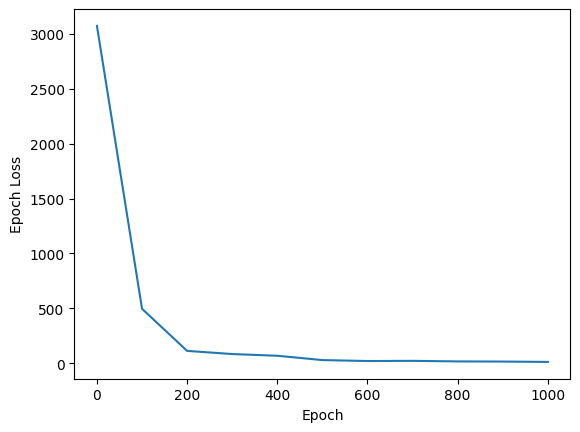
\includegraphics[width=0.8\linewidth]{loss.png}
    \caption{Verlust nach Epoche des Trainings}
    \label{fig:enter-label}
\end{figure}
Zum Trainieren des Neuronalen Netzes wurden ebenfalls PyTorch-intrinsische Funktionen verwendet. Es wurde die Methode des \textbf{überwachten Lernes} verwendet. Bei dieser Methode werden gelabelte Daten verwendet. Dies bedeutet, dass dem Modell stets zu jedem Datenvektor die korrekte Transpirationsfläche mit angegeben wurde, damit diese beim Berechnen des Fehlers berücksichtigt werden können und das Netz entsprechend angepasst wird.
\begin{figure}
    \centering
    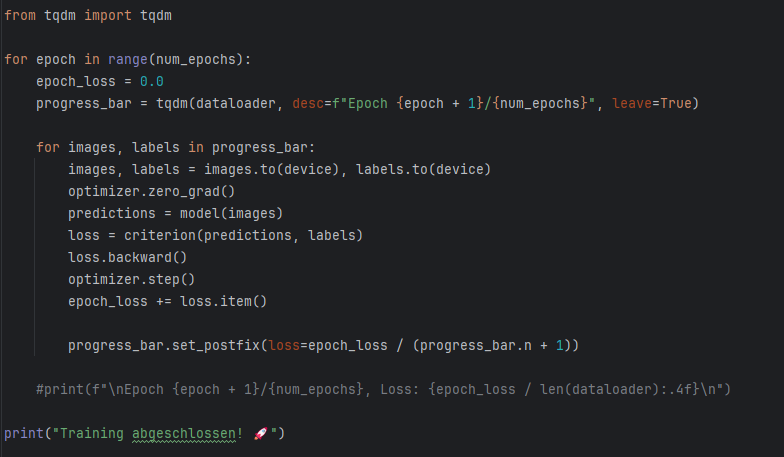
\includegraphics[width=1\linewidth]{Screenshot 2025-03-30 171125.png}
    \caption{Trainingsalgorithmus}
    \label{fig:enter-label}
\end{figure}
In Abbildung 15 ist die Implementierung des entsprechenden Trainingsalgorithmus zu sehen. Um die visuelle Verständlichkeit während des Trainingsvorgangs zu verbessern, wurde aus der \textbf{TQDM} Bibliothek die Funktion zum Darstellen von Ladebalken in CLI-Umgebungen verwendet. Als Optimierer wurde aufgrund der breiten Anwendung die \textbf{Adam Optimizer} gewählt.
\subsection{Verwendete Hardware und Laufzeit}
Für das Projekt wurde ein Server mit einem 16-Kern AMD Ryzen 3950X und einer NVIDIA GTX 1080 Ti verwendet. Der Prozessor hat 32 Hardware-Threads zur Verfügung und die Grafikkarte hat mittels ihrer 3584 CUDA-Kerne gerechnet. Beide Komponenten sind wassergekühlt, um eine möglichst temperaturunabhängige Leistungsabgabe zu gewährleisten. Insgesamt wurde das Modell auf 1000 Epochen trainiert. Das Training hatte eine Gesamtlaufzeit von ca. 33 Minuten.
\section{Fazit}
\begin{figure}
    \centering
    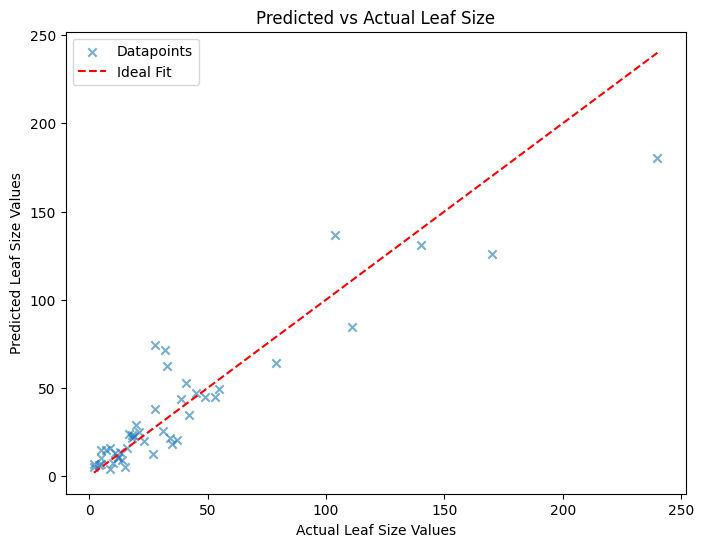
\includegraphics[width=0.8\linewidth]{scatter.png}
    \caption{Vergleich der Modell-Vorhersage zum realen Wert}
    \label{fig:enter-label}
\end{figure}
Ziel dieser Arbeit war es, mittels Bildanalyse eine geeignete Metrik zu finden, um den Wasserbedarf einer Zuckerrübenpflanze zu bestimmen. Hierbei wurde ein entsprechender Datensatz gewählt, welcher konsistent und themenbezogen war. Es konnte nachgewiesen werden, dass mit einer genügenden Datenlage und entsprechender Trainingshardware sowie dem entsprechenden Modell eines neuronalen Netzes durchaus eine gute Einschätzung der Transpirationsfläche erstellbar ist. Die Transpirationsfläche ist stochastisch wiederum an das Alter der Pflanze gekoppelt, womit eine zusätzliche Metrik erhoben werden kann. Zu beachten ist es allerdings, dass es sich dabei um ein theoretisches Alter nach dauerhaftem Wachstum handelt. Da es sich bei der Wasseraufnahme und dem Wasserverbrauch ohnehin um natürlich bedingte stochastische Prozesse handelt, ist der Fehler für die Erhebung der benötigten Wassermenge durchaus als trivial zu bewerten. \newline \par Im Bezug auf die Skalierung von Vertical Farming wurde das container-basierte Vertical Farming untersucht, welches durch seinen modularen Aufbau sowie extreme Standortunabhängigkeit sich nach dem Schluss dieser Arbeit sehr gut eignet, um Vertical Farms aufzubauen, die in íhrer Größe variabel sein müssen.
\section{Ausblick}
In der Suche nach einem Anschluss an diese Arbeit ist definitiv die Verbesserung der Datenlage der primäre Anhaltspunkt. Einerseits wären mehr Bilder von den Setzlingen besser, um die Genauigkeit zu erhöhen, und andererseits wäre es von großem Nutzen, die Messung der Transpirationsfläche der Trainingsdaten mit einem besseren Verfahren als der subjektiven Schätzung zweier Personen durchzuführen. Problematisch ist hierbei einerseits der menschliche Bias bei der Einschätzung von Größen, aber auch die Kontextabhängigkeit. Außerdem wäre ein passendes Experiment denkbar, bei dem von dem beschriebenen Modell dieser Arbeit ausgegangen wird, um die benötigte Wassermenge zu bestimmen. Dieses Ergebnis könnte man daraufhin gegebenenfalls mit anderen Modellen oder Algorithmen beziehungsweise klassischen approximativen Methoden vergleichen. Außerdem wäre es sehr interessant, einen entsprechenden Hardwareansatz zu verfolgen und das komplette System als Prototyp zu implementieren. Dazu würde dann auch die Art und Weise, wie die Bilder geschossen werden, von Relevanz sein.
\newpage
\section{Quelltext}
\subsection{train.py}
\begin{minted}[mathescape, linenos]{python}
import os
import torch
import torch.nn as nn
import torch.optim as optim
from PIL import Image
import torchvision.transforms as transforms
from torch.utils.data import Dataset, DataLoader

device = torch.device("cuda" if torch.cuda.is_available() else "cpu")
print(f"Using device: {device}")

def get_size_from_filename(filename):
    return float(filename.split(".")[0].split("_")[1])

class LeafAgeDataset(Dataset):
    def __init__(self, image_folder):
        self.image_folder = image_folder
        self.files = os.listdir(image_folder)
        self.transform = transforms.Compose([
            transforms.ToTensor(),
            transforms.Normalize(mean=[0.5, 0.5, 0.5], std=[0.5, 0.5, 0.5])
        ])

    def __len__(self):
        return len(self.files)

    def __getitem__(self, idx):
        file = self.files[idx]
        img = Image.open(os.path.join(self.image_folder, file))
        img_tensor = self.transform(img)

        age = get_size_from_filename(file)
        return img_tensor, torch.tensor([age], dtype=torch.float32)


dataset = LeafAgeDataset("destination_images")
dataloader = DataLoader(dataset, batch_size=16, shuffle=True)


class AgePredictionCNN(nn.Module):
    def __init__(self):
        super(AgePredictionCNN, self).__init__()
        self.conv_layers = nn.Sequential(
            nn.Conv2d(3, 32, kernel_size=3, stride=1, padding=1),
            nn.ReLU(),
            nn.MaxPool2d(2, 2),
            nn.Conv2d(32, 64, kernel_size=3, stride=1, padding=1),
            nn.ReLU(),
            nn.Conv2d(64, 64, kernel_size=3, stride=1, padding=1),
            nn.ReLU(),
            nn.AdaptiveAvgPool2d((4, 4))
        )
        self.fc_layers = nn.Sequential(
            nn.Flatten(),
            nn.Linear(64 * 4 * 4, 64),
            nn.ReLU(),
            nn.Linear(64, 32),
            nn.ReLU(),
            nn.Linear(32, 16),
            nn.ReLU(),
            nn.Linear(16, 1)
        )

    def forward(self, x):
        x = self.conv_layers(x)
        return self.fc_layers(x)

model = AgePredictionCNN().to(device)
print(model)
criterion = nn.MSELoss()
optimizer = optim.Adam(model.parameters(), lr=0.001)

num_epochs = 1000
print(torch.cuda.is_available())

from tqdm import tqdm

for epoch in range(num_epochs):
    epoch_loss = 0.0
    progress_bar = tqdm(dataloader, desc=f"Epoch {epoch + 1}/{num_epochs}", leave=True)

    for images, labels in progress_bar:
        images, labels = images.to(device), labels.to(device)
        optimizer.zero_grad()
        predictions = model(images)
        loss = criterion(predictions, labels)
        loss.backward()
        optimizer.step()
        epoch_loss += loss.item()

        progress_bar.set_postfix(loss=epoch_loss / (progress_bar.n + 1))

    #print(f"\nEpoch {epoch + 1}/{num_epochs}, Loss: {epoch_loss / len(dataloader):.4f}\n")

torch.save(model, "model.pth")
print("Training abgeschlossen!")
\end{minted}
\subsection{test.py}
\begin{minted}[mathescape, linenos]{python}
import os

import torch
from PIL import Image
from torch import device, nn
from torchvision import transforms

class AgePredictionCNN(nn.Module):
    def __init__(self):
        super(AgePredictionCNN, self).__init__()
        self.conv_layers = nn.Sequential(
            nn.Conv2d(3, 32, kernel_size=3, stride=1, padding=1),
            nn.ReLU(),
            nn.MaxPool2d(2, 2),
            nn.Conv2d(32, 64, kernel_size=3, stride=1, padding=1),
            nn.ReLU(),
            nn.Conv2d(64, 64, kernel_size=3, stride=1, padding=1),
            nn.ReLU(),
            nn.AdaptiveAvgPool2d((4, 4))
        )
        self.fc_layers = nn.Sequential(
            nn.Flatten(),
            nn.Linear(64 * 4 * 4, 64),
            nn.ReLU(),
            nn.Linear(64, 32),
            nn.ReLU(),
            nn.Linear(32, 16),
            nn.ReLU(),
            nn.Linear(16, 1)
        )

    def forward(self, x):
        x = self.conv_layers(x)
        return self.fc_layers(x)
def get_size_from_filename(filename):
    return float(filename.split(".")[0].split("_")[1])

device = torch.device("cuda" if torch.cuda.is_available() else "cpu")
print(f"Using device: {device}")

model = torch.load("model.pth", map_location=device)
model.eval()

def predict_image(image_name):
    image_path = os.path.join("test_images", image_name)

    image = Image.open(image_path)

    transform = transforms.Compose([
        transforms.ToTensor(),
        transforms.Normalize(mean=[0.5, 0.5, 0.5], std=[0.5, 0.5, 0.5])
    ])

    image_tensor = transform(image).unsqueeze(0).to(device)

    model.eval()

    with torch.no_grad():
        predicted_age = model(image_tensor).item()

    print(f"Predicted transpiration area for the image {image_name}: {predicted_age:.2f} real transpiration area: {get_size_from_filename(image_name)}")

for image in os.listdir("test_images"):
    predict_image(image)
\end{minted}
Das gesamte Projekt liegt in dem persönlichen GitHub-Repository von Sten Heimbrodt unter \newline\hyperlink{https://github.com/gespel/leaf-age-guesser}{https://github.com/gespel/leaf-age-guesser}